\documentclass[border=2pt]{standalone}
\usepackage[utf8]{inputenc} % Required for inserting images
\usepackage{tikz}
\usetikzlibrary{shapes.geometric, arrows}

% -------------------------defining nodes 
\tikzstyle{startstop} = [rectangle, rounded corners, minimum width=3cm, minimum height=1cm,
text centered, draw = black, fill=blue!30]
\tikzstyle{io} = [trapezium, trapezium left angle =70, trapezium right angle = 110,
minimum width= 3cm, minimum height=1cm, text centered, draw=black, fill=blue!30]
\tikzstyle{process} = [rectangle, minimum width = 3cm, minimum height = 1cm,
text centered, , text width=4cm,draw=black, fill=gray!30]
\tikzstyle{decision} = [diamond, minimum width = 3cm, minimum height = 1cm,
text centered, , text width=4cm, draw=black, fill=cyan!30]
\tikzstyle{reject} = [rectangle, minimum width= 1cm, minimum height = 1cm, 
text centered, , text width=3cm, draw=black, fill=red!30]
\tikzstyle{accept} = [rectangle, minimum width= 1cm, minimum height = 1cm, 
text centered, , text width=3cm, draw=black, fill=green!30]
% -------------------------defining connectors
\tikzstyle{arrow} = [thick,->, >=stealth]
\tikzstyle{line} = [thick,-,>=stealth]
\begin{document}

% ------------------------- tikz image (flow chart)
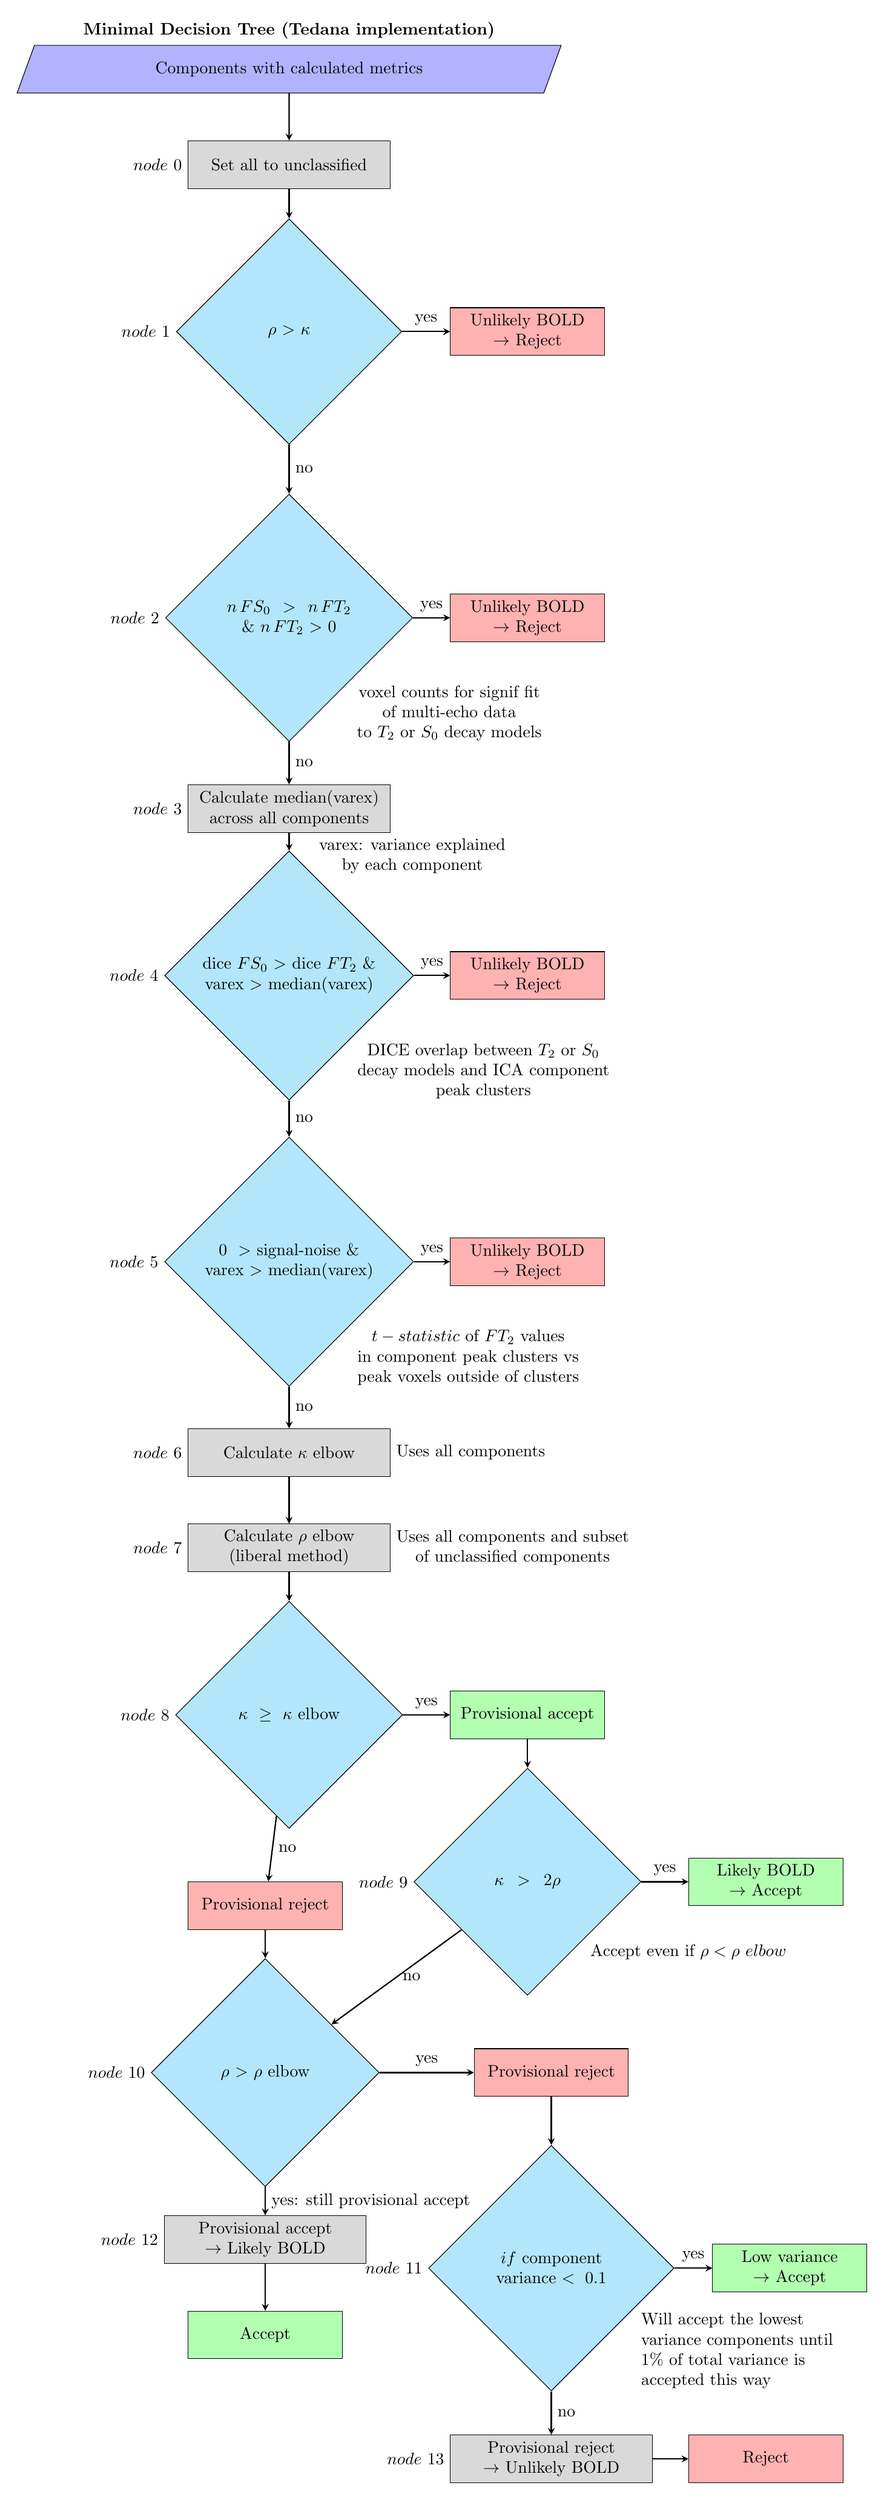
\begin{tikzpicture}[node distance = 2cm]

% ------------------------- nodes -------------------------


% ----- node: input
\node(input) [io,label={90:\textbf{Minimal Decision Tree (Tedana implementation)}}] {Components with calculated metrics};
% ----- node: 0
\node(0)[process, below of=input,label={180:$node\ 0$}]{Set all to unclassified};
% ----- node: 1
\node(1)[decision, below of=0,label={180:$node\ 1$}, yshift=-1.5cm]{$\rho$ $>$ $\kappa$};
\node(rej0)[reject, right of=1, xshift=3cm]{Unlikely BOLD $\rightarrow$ Reject};
% ----- node: 2
\node(2)[decision, below of=1,label={180:$node\ 2$}, label={[align=center] 315: voxel counts for signif fit\\of multi-echo data\\to $T_2$ or $S_0$ decay models}, yshift=-4.0cm]{$n \, FS_0 \, > \, n \, FT_2$ \& $n \,FT_2$ $>$ 0};
\node(rej1)[reject, right of=2, xshift=3cm]{Unlikely BOLD $\rightarrow$ Reject};
% ----- node: 3
\node(3)[process, below of=2, label={180:$node\ 3$}, label={[align=center] 315: varex: variance explained\\by each component}, yshift=-2.0cm]{Calculate median(varex) across all components};
% ----- node: 4
\node(4)[decision, below of=3,label={180:$node\ 4$},label={[align=center] 315:DICE overlap between $T_2$ or $S_0$\\decay models and ICA component\\peak clusters}, yshift=-1.5cm]{dice $FS_0$ $>$ dice $FT_2$ \& varex $>$ median(varex)
};
\node(rej2)[reject, right of=4, xshift=3cm]{Unlikely BOLD $\rightarrow$ Reject};
% ----- node: 5
\node(5)[decision, below of=4,label={180:$node\ 5$}, label={[align=center] 315: $t-statistic$ of $FT_2$ values\\in component peak clusters vs\\peak voxels outside of clusters}, yshift=-4.0cm]{ $0 \, >$ signal-noise \&  varex $>$ median(varex)};
\node(rej3)[reject, right of=5, xshift=3cm]{Unlikely BOLD  $\rightarrow$ Reject};
% ----- node: 6
\node(6)[process, below of=5, label={180:$node\ 6$}, label={0: Uses all components}, yshift=-2.0cm]{Calculate $\kappa$ elbow};
% ----- node: 7
\node(7)[process, below of=6, label={180:$node\ 7$}, label={[align=center] 0: Uses all components and subset\\of unclassified components}]{Calculate $\rho$ elbow\\(liberal method)};
% ----- node: 7
\node(8)[decision, below of=7,label={180:$node\ 8$}, yshift=-1.5cm]{$\kappa \geq \kappa$ elbow};
\node(rej8)[reject, below of=8, xshift=-0.5cm, yshift=-2cm]{Provisional reject};
\node(rej4)[accept, right of=8, xshift=3cm, yshift=0cm]{Provisional accept};
% ----- node: 8
\node(9)[decision, below of=rej4,label={180:$node\ 9$},label={315: Accept even if $\rho < \rho\ elbow$},yshift=-1.5cm]{$\kappa > 2\rho$  };
\node(rej5)[accept, right of=9, xshift=3cm]{Likely BOLD $\rightarrow$ Accept};
% ----- node: 9
\node(10)[decision, below of=rej8,label={180:$node\ 10$}, yshift=-1.5cm]{ $\rho$ $>$ $\rho$ elbow};
\node(rej6)[reject, right of=10, xshift=4cm]{Provisional reject};
% ----- node: 10
\node(11)[decision, below of=rej6,label={180:$node\ 11$},label={[align=left] 335: Will accept the lowest\\variance components until\\1\% of total variance is\\accepted this way}, yshift=-2.1cm]{$if$ component variance $<0.1$};%--check in kundu
\node(rej7)[accept, right of=11, xshift=3cm]{Low variance $\rightarrow$ Accept};
% ----- node: 11
\node(12)[process, below of=10,label={180:$node\ 12$},yshift=-1.5cm]{Provisional accept $\rightarrow$ Likely BOLD};
\node(rej12)[accept, below of=12]{Accept};
% ----- node: 12
\node(13)[process, below of=11,label={180:$node\ 13$}, yshift=-2.0cm]{Provisional reject $\rightarrow$ Unlikely BOLD};
\node(rej13)[reject, right of=13, xshift=2.5cm]{Reject};

% ------------------------- connections -------------------------
% draw[x](origin)--node[anchor=position]{text}(destination);
\draw[arrow](input)--(0);
\draw[arrow](0)--(1);
\draw[arrow](1)--node[anchor=south, right=0] {no} (2);
\draw[arrow](2)--node[anchor=south, right=0] {no} (3);
\draw[arrow](3)--(4);
\draw[arrow](4)--node[anchor=south, right=0] {no} (5);
\draw[arrow](5)--node[anchor=south, right=0] {no} (6);
\draw[arrow](6)--(7);
\draw[arrow](7)--(8);
% \draw[arrow](8)--(9);
\draw[arrow](9)--node[anchor=south, right=0] {no} (10);
% \draw[arrow](10)--(11);
\draw[arrow](10)--node[anchor=south, right=0] { yes: still provisional accept} (12);
\draw[arrow](11)--node[anchor=south, right=0] {no} (13);
\draw[arrow](1)--node[anchor=south] {yes} (rej0);
\draw[arrow](2)--node[anchor=south] {yes} (rej1);
\draw[arrow](4)--node[anchor=south] {yes} (rej2);
\draw[arrow](5)--node[anchor=south] {yes} (rej3);% check on kundu
\draw[arrow](8)--node[anchor=south] {yes} (rej4);
\draw[arrow](8)--node[anchor=south, right=0] {no} (rej8);
\draw[arrow](rej4)--(9);
\draw[arrow](rej6)--(11);
\draw[arrow](rej8)--(10);
\draw[arrow](9)--node[anchor=south] {yes} (rej5);
% \draw[arrow](rej5)--(10);
\draw[arrow](10)--node[anchor=south] {yes} (rej6);
\draw[arrow](11)--node[anchor=south] {yes} (rej7);
\draw[arrow](12)--(rej12);
\draw[arrow](13)--(rej13);

\end{tikzpicture}
\end{document}
